\chapter{仿真实验与一致性测试}
\label{cha:evaluate}


\section{本章引言}
本章主要对RSCP-iBGP系统的功能和性能进行了测试评价、对新系统下的新协议进行了一致性测试。功能验证方面,通过设计合理的网络拓扑,验证RSCP-iBGP系统,实现了路由策略的集中配置、路由存储的集中优化、在路由计算的过程中基于全部路由且不存在因为MED不可比引起路由震荡等功能。性能评价方面,主要关注大规模路由下的路由存储的大小和收敛时间的快慢。本文提出的RSCP-iBGP新系统实际上对iBGP协议进行了改动,对RSCP-iBGP新系统下的新协议通过TTCN-3测试例进行一致性测试,很好地验证了RSCP-iBGP系统功能实现与设计的一致性。

\section{RSCP-iBGP系统功能验证实验}

第3章的例子都跑一边,如何证明你的系统的正确性?
实验方面RCP和RFCP是怎么实现的?

\subsection{路由策略集中配置}

\subsection{路由存储集中优化}

\subsection{基于全部路由且无MED值引起的路由震荡}


\section{RSCP-iBGP系统性能评价实验}

\subsection{大规模路由信息下的路由存储}

\subsection{路由收敛时间评估}


\begin{figure}
  \centering
  % Requires \usepackage{graphicx}
  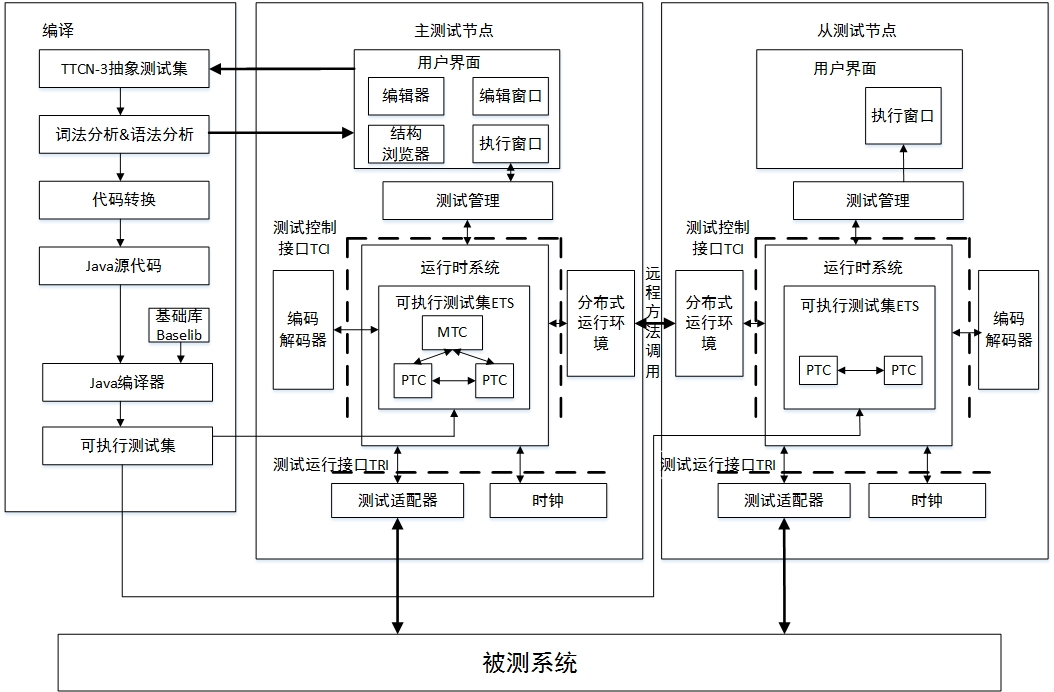
\includegraphics[width=0.75\textwidth]{pitsv3}
  \caption{PitSv3系统的体系结构\cite{pitsv3}}
  \label{fig:pitsv3}
\end{figure}


\section{协议的一致性测试}
\subsection{测试平台介绍}
测试平台使用协议测试系统工具PITSv3,,PITSv3内通过主测试部件和多个从测试部件,来模拟测试系统多网口的情况,每个测试部件可以连接一个真实的虚拟路由器,以此来构建拓扑,实现测试。PITSv3系统的体系结构见图\ref{fig:pitsv3}。
\subsection{一致性测试需求}

对RSCP-iBGP系统的测试主要分两个测试组:对自治系统内的边界路由器进行测试、对自治系统内的Route-Server进行测试。具体的测试需求加下。

测试例:新增加的传输Weight路径属性的UPDATE报文!


对自治系统内的边界路由器进行测试:
\begin{itemize}
  \item 与自治系统内的Route-Server作为iBGP Peer时,进行邻居建连测试、对等体断连测试、前缀报文交互(路由宣告)测试;
  \item 与自治系统外的边界路由器作为eBGP Peer时,进行邻居建连测试、对等体断连测试、前缀报文交互(路由宣告)测试。
\end{itemize}

对自治系统内的Route-Server进行测试:
\begin{itemize}
  \item 与自治系统内的边界路由器作为iBGP Peer时,进行邻居建连测试、对等体断连测试、前缀报文交互(路由宣告)测试。
\end{itemize}




\subsection{测试集设计}

根据测试需求设计的测试集如表\ref{tab:test}。
% Please add the following required packages to your document preamble:
% \usepackage{multirow}
\begin{table}[h]
\centering
\caption{RSCP-iBGP系统的一致性测试集}
\label{tab:test}
\begin{tabular}{|l|l|l|}
\hline
测试组 & 测试用例 & 测试目的 \\ \hline
\multirow{6}{*}{\begin{tabular}[c]{@{}l@{}}对边界路由器\\ 进行测试\end{tabular}} & 与iBGP对等体建连 & \begin{tabular}[c]{@{}l@{}}边界路由器向Route-Server发送OPEN报文,\\ 请求建立连接\end{tabular} \\ \cline{2-3}
 & 与iBGP对等体断连 & \begin{tabular}[c]{@{}l@{}}Route-Server连续3次未收到边界路由器\\ 的KEEPALIVE断连\end{tabular} \\ \cline{2-3}
 & 与iBGP对等体前缀报文交互 & \begin{tabular}[c]{@{}l@{}}Route-Server向边界路由器发送路由更新信息,\\ 边界路由器将其转发至全部的EBGP邻居\end{tabular} \\ \cline{2-3}
 & 与eBGP对等体建连 & \begin{tabular}[c]{@{}l@{}}边界路由器向eBGP对等体发送OPEN报文,\\ 请求建立连接\end{tabular} \\ \cline{2-3}
 & 与eBGP对等体断连 & \begin{tabular}[c]{@{}l@{}}eBGP对等体连续3次未收到边界路由器\\ 的KEEPALIVE断连\end{tabular} \\ \cline{2-3}
 & 与eBGP对等体前缀报文交互 & \begin{tabular}[c]{@{}l@{}}eBGP对等体向边界路由器发送路由更新信息,\\ \\ 边界路由器将其转发至Route-Server\end{tabular} \\ \hline
\multirow{3}{*}{\begin{tabular}[c]{@{}l@{}}对Route-Server\\ 进行测试\end{tabular}} & 与iBGP对等体建连 & \begin{tabular}[c]{@{}l@{}}Route-Server向边界路由器发送OPEN报文,\\ 请求建立连接\end{tabular} \\ \cline{2-3}
 & 与iBGP对等体断连 & \begin{tabular}[c]{@{}l@{}}边界路由器连续3次未收到Route-Server\\ 的KEEPALIVE断连\end{tabular} \\ \cline{2-3}
 & 与iBGP对等体前缀报文交互 & \begin{tabular}[c]{@{}l@{}}边界路由器向Route-Server发送路由更新信息,\\ \\ Route-Server将最优路由转发至全部的iBGP邻居\end{tabular} \\ \hline
\end{tabular}
\end{table}


\subsection{测试结果及分析}

\section{本章小结}

本章主要对RSCP-iBGP系统的进行了功能验证、性能评价以及一致性测试。通过本章的仿真实验和协议测试,本文实现的RSCP-iBGP系统在性能实现上达到了最初的设计目标:基于全部路由进行路由计算,集合缩小式的新型路由算法也能避免MED不可比引起的路由震荡,路由策略集中配置,路由表在集中平台上存储优化,RSCP-iBGP系统上Route-Server的路由计算次数和路由存储大小均优化了一个数量级。
